\documentclass[a4paper,11pt,titlepage]{jarticle}
\usepackage[dvipdfmx]{graphicx}
\usepackage{listings}
\usepackage{amsmath}
\usepackage{fancybox,ascmac}
\usepackage{url}

\title{知能情報実験II(第14回):ロジスティックモデル}
\author{175751C 宮城孝明}
\date{\today}

\begin{document}
\maketitle
\tableofcontents
\clearpage

\section{分岐図}
\subsection{プログラムのソースコード(python)}
\lstinputlisting[language=python, numbers=left, breaklines=true, basicstyle=\ttfamily\footnotesize,
  frame=single, caption=branch\_code, label=sample]{branch.py}
\subsection{プログラムのソースコード(C)}
\lstinputlisting[language=C, numbers=left, breaklines=true, basicstyle=\ttfamily\footnotesize,
  frame=single, caption=branch\_code, label=sample]{branch.c}
\subsection{結果と考察}
図1では,最大増加率rが増えることにより,Xnも増えていっている.それは,第n世代(親世代)の個体数がrに従って,
増加するということを表している.さらに,一定の曲線を描いているたえ,親世代の個体数は一定に推移していると考えられる.
しかし,rが3を超えたあたりから,線が2つに分岐している.これは,rの増加で親の個体数が増得たり,減ったりしている
ことを示している.そして,3.6以降は値がバラバラになっているため,ここからは親の個体数の変動が激しいと
考えられる.
\begin{figure}[htbp]
  \centering
  \includegraphics[width=80mm]{c_branch.png}
  \label{branch}\\
  \caption{branch}
\end{figure}



\section{リアプノフ指数}
\subsection{プログラムのソースコード(python)}
\lstinputlisting[language=python, numbers=left, breaklines=true, basicstyle=\ttfamily\footnotesize,
  frame=single, caption=branch\_code, label=sample]{Lyapunov.py}
\subsection{プログラムのソースコード(C)}
\lstinputlisting[language=C, numbers=left, breaklines=true, basicstyle=\ttfamily\footnotesize,
  frame=single, caption=branch\_code, label=sample]{lyapunov.c}
\subsection{結果と考察}
リアプノフ指数は,カオス性質が見られるデータ(例 脳波)を解析するために用いられる計算式である.\par
カオス性質とは,初期条件によって後の経過に影響を与える性質のことである.
今回の実験も初期の値に大きな影響を受けるため,この式が用いられていると思われる.\par
rが3.5からy軸が0を越えていることから,やはり親個数の激しい変動が関係しているのだと考えられる.
\begin{figure}[htbp]
  \centering
  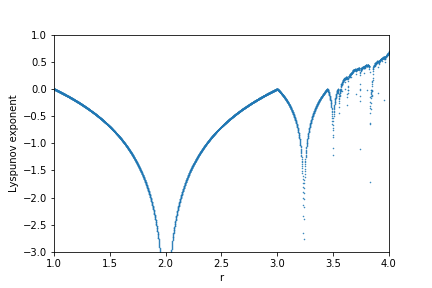
\includegraphics[width=80mm]{x_lyapunov.png}
  \label{Lyapunov}\\
  \caption{Lyapunov}
\end{figure}

\section{特別課題}
図1で作成した分岐図を拡大し,より細かくみるために作成し他のが図3の3周期の窓である.3.830から3.855
の間に隙間が存在する.そのため,このような形になる.つまり,ここの間には親世代の個体数が3本線の間を移動すると
予測できる.さらに,よく見てみると真ん中の線は2本に別れ,さらに2本に別れている.そして,真ん中に隙間みたいなのができている.
これは,図1のグラフと似ている.この隙間中には,何個も同じ形のグラフがあるのではないかと予測する.

\begin{figure}[htbp]
  \centering
  \includegraphics[width=80mm]{3priod.png}
  \label{3周期の窓}\\
  \caption{3周期の窓}
\end{figure}

\section{参考文献}
\begin{thebibliography}{99}
	\bibitem{知能情報実験} 知能情報実験II : ロジスティックモデル; 國田樹(琉球大学工学部知能情報コース) 2019年1月
\end{thebibliography}

\end{document}
